%%%%%%%%%%%%%%%%%%%%%%%%%%%%%%%%%%%%%%%%%%%%%%%%%%%%%%%%%%%%%%%%%%%%%%%%%%%%
% AGUtmpl.tex: this template file is for articles formatted with LaTeX2e,
% Modified March 2013
%
% This template includes commands and instructions
% given in the order necessary to produce a final output that will
% satisfy AGU requirements.
%
% PLEASE DO NOT USE YOUR OWN MACROS
% DO NOT USE \newcommand, \renewcommand, or \def.
%
% FOR FIGURES, DO NOT USE \psfrag or \subfigure.
%
%%%%%%%%%%%%%%%%%%%%%%%%%%%%%%%%%%%%%%%%%%%%%%%%%%%%%%%%%%%%%%%%%%%%%%%%%%%%
%
% All questions should be e-mailed to latex@agu.org.
%
%%%%%%%%%%%%%%%%%%%%%%%%%%%%%%%%%%%%%%%%%%%%%%%%%%%%%%%%%%%%%%%%%%%%%%%%%%%%
%
% Step 1: Set the \documentclass
%
% There are two options for article format: two column (default)
% and draft.
%
% PLEASE USE THE DRAFT OPTION TO SUBMIT YOUR PAPERS.
% The draft option produces double spaced output.
%
% Choose the journal abbreviation for the journal you are
% submitting to:

% jgrga JOURNAL OF GEOPHYSICAL RESEARCH
% gbc   GLOBAL BIOCHEMICAL CYCLES
% grl   GEOPHYSICAL RESEARCH LETTERS
% pal   PALEOCEANOGRAPHY
% ras   RADIO SCIENCE
% rog   REVIEWS OF GEOPHYSICS
% tec   TECTONICS
% wrr   WATER RESOURCES RESEARCH
% gc    GEOCHEMISTRY, GEOPHYSICS, GEOSYSTEMS
% sw    SPACE WEATHER
% ms    JAMES
% ef    EARTH'S FUTURE
%
%
%
% (If you are submitting to a journal other than jgrga,
% substitute the initials of the journal for "jgrga" below.)

\documentclass[draft,grl]{AGUTeX}
% To create numbered lines:

% If you don't already have lineno.sty, you can download it from
% http://www.ctan.org/tex-archive/macros/latex/contrib/ednotes/
% (or search the internet for lineno.sty ctan), available at TeX Archive Network (CTAN).
% Take care that you always use the latest version.

% To activate the commands, uncomment \usepackage{lineno}
% and \linenumbers*[1]command, below:

\usepackage{lineno}
\usepackage{amssymb}
\usepackage{amsmath}
\usepackage{textcomp}
\usepackage[super]{nth}
\usepackage{tabularx}
\usepackage{multirow}
\usepackage{bm}
\usepackage{color} 

\linenumbers*[1]

%  To add line numbers to lines with equations:
%  \begin{linenomath*}
%  \begin{equation}
%  \end{equation}
%  \end{linenomath*}
%%%%%%%%%%%%%%%%%%%%%%%%%%%%%%%%%%%%%%%%%%%%%%%%%%%%%%%%%%%%%%%%%%%%%%%%%
% Figures and Tables
%
%
% DO NOT USE \psfrag or \subfigure commands.
%
%  Figures and tables should be placed AT THE END OF THE ARTICLE,
%  after the references.
%
%  Uncomment the following command to include .eps files
%  (comment out this line for draft format):
\usepackage[final]{graphicx}
%
%  Uncomment the following command to allow illustrations to print
%   when using Draft:
%  \setkeys{Gin}{draft=false}
%
% Substitute one of the following for [dvips] above
% if you are using a different driver program and want to
% proof your illustrations on your machine:
%
% [xdvi], [dvipdf], [dvipsone], [dviwindo], [emtex], [dviwin],
% [pctexps],  [pctexwin],  [pctexhp],  [pctex32], [truetex], [tcidvi],
% [oztex], [textures]
%
% See how to enter figures and tables at the end of the article, after
% references.
%
%% ------------------------------------------------------------------------ %%
%
%  ENTER PREAMBLE
%
%% ------------------------------------------------------------------------ %%

% Author names in capital letters:
\authorrunninghead{DAY ET AL.}

% Shorter version of title entered in capital letters:
\titlerunninghead{SOUTH FLOOD-NORTH DROUGHT IN MEIYU AND JET STATS}

%Corresponding author mailing address and e-mail address:
\authoraddr{Corresponding author: Jesse Day, University of California Berkeley, Department of Earth and Planetary Science, College of Letters and Science; 307 McCone Hall, Berkeley, CA 94720, USA. (jessed@berkeley.edu)}

\begin{document}

%% ------------------------------------------------------------------------ %%
%
%  TITLE
%
%% ------------------------------------------------------------------------ %%


\title{A 57-year Catalog of Meiyu Front Statistics: Relation to Jet Behavior and Signal of the ``South Flood-North Drought''}

%% ------------------------------------------------------------------------ %%
%
%  AUTHORS AND AFFILIATIONS
%
%% ------------------------------------------------------------------------ %%


%Use \author{\altaffilmark{}} and \altaffiltext{}

% \altaffilmark will produce footnote;
% matching \altaffiltext will appear at bottom of page.

\authors{Jesse A. Day\altaffilmark{1},
Jacob Edman\altaffilmark{1}, John C. H. Chiang\altaffilmark{1}, Inez Fung \altaffilmark{1}, and
Weihan Liu\altaffilmark{1}}

\altaffiltext{1}{Department of Earth and Planetary Science, University of California Berkeley, Berkeley, California, USA.}

%% ------------------------------------------------------------------------ %%
%
%  ABSTRACT
%
%% ------------------------------------------------------------------------ %%

% >> Do NOT include any \begin...\end commands within
% >> the body of the abstract.

%Needs to be 150 words or less - currently at 179.
\begin{abstract}
A growing body of literature claims a change in summer rainfall distribution over China after the late 1970s (the ``South Flood North Drought''). In these months, rainfall characteristically occurs along zonal bands with a meridional tilt (the Meiyu Front). We construct a novel database that tracks all occurrences of frontal rainfall over China on each day from 1951 to 2007 from APHRODITE rain gauge data, and reports their latitude, strength, tilt and width. An unprecedented Meiyu climatology is obtained. In addition, the latitude of frontal events is known to correspond to the position of the tropospheric jet. Therefore, we search for correspondence between front and jet position, and coupled changes in behavior with time. Two robust changes are observed in front behavior between the time periods 1951-1979 and 1980-2007: 1) A significant decrease in the frequency of pre-Meiyu (May) frontal events after 1979 and 2) a southward shift in late season Meiyu events (mid-July to August) found both in the front and jet databases. Our results hold the promise of coupling regional climate change to \nth{21} century global change.

%2 claims:
% 1. South-flood, north-drought pattern is a change in location, frequency and intensity of Meiyu events
% 2. These changes in the meiyu are reflected in jet changes (i.e. they are driven by planetary scale things) 

\end{abstract}

\begin{article}

%% ------------------------------------------------------------------------ %%

%%  THINGS THAT ARE MISSING  %%
% Need to produce Figure 2 (Meiyu frequency changes and rainfall changes between 1951-1979 and 1980-2007 + statistical significance).

%% ------------------------------------------------------------------------ %%

\section{Introduction}
 
 	China receives about 60\% of its rainfall from May to August, known collectively as the East Asian summer monsoon. The period of peak rainfall within this monsoon lasts roughly from early June to mid-July (usually referred to as ``Meiyu Season'') features a northward-migrating front known as the Meiyu front (lit. ``Plum rains,'' referring to the spectacular growth of plum blossoms in central China after the onset of heavy rains). The corresponding rainy seasons in Japan and Korea are known as Baiu and Changma respectively. A growing volume of evidence suggests a shift in mean rainfall patterns over China beginning in the late 1970s, with increased flooding in the south and droughts in the north (the ``South Flood North Drought'') \citep{Hu1997,Gong2002}. A permanent change would have major humanitarian impacts on the densely-populated eastern Chinese plain, where a sizable fraction of the population depends on agriculture. Northern China suffers from substantial depletion of freshwater resources along with increasing demand \citep{Currell2012,Gleeson2012}. The Chinese government has already embarked on a project to reroute water from the Yangtze River to northern China, the South-North Water Transfer Project (\textit{nanshui beidiao gongcheng}), which is expected to become the most expensive hydraulic engineering project ever undertaken and will entail massive human and environmental impact \citep{Magee2011}.
 
	Although summer rainfall in East Asia is referred to as a monsoon, the climatology bears little resemblance to its Indian counterpart or other monsoon circulations worldwide \citep{Ding2005}. Whereas understanding of tropical monsoons has progressed greatly via theoretical studies \citep{Plumb1992,Prive2007,Bordoni2008}, the dynamics that favor the existence of frontal convection over East Asia in summer remain a point of debate \citep{Sampe2010,Chen2014}. The migration of the Meiyu front entails shifts in large-scale circulation \citep{Chen2004}. The seasonal mean progression of the Meiyu Front has been shown to feature three broad stages of behavior, each with a preferred front latitude, and abrupt transitions from one state to the next \citep{Ding2005}. Furthermore, anomalies in Meiyu front latitude produce corresponding rainfall anomalies \citep{Kosaka2011}. Therefore, a long-term change in rainfall r\'egime such as the South Flood-North Drought should be attributable to a change in the characteristics of Meiyu events, such as a shift in latitude, a change in intensity or an earlier or later transition from one stage to the next.
	
	In pursuit of this aim, we have developed a 57-year climatology (1951-2007) of frontal events in China based on the APHRODITE rain gauge product (described below). We develop a convergent fitting algorithm of daily rainfall maps which returns information about the position and strength of the front, as described in greater detail below. A few previous studies have discussed the statistics of the Meiyu front on decadal and even centennial time scales \citep{Chen2004,Ge2008,Xu2009}, but to our knowledge no author has compiled a multi-decadal daily catalog of events. We use this database to clarify the spatial and temporal characteristics of the South Flood-North Drought, and present it as a tool for future East Asian monsoon research.
		
	We focus on links between the behavior of the Meiyu front and subtropical jet, which plays an essential and complex role in East Asian climate. In a region with a sharp temperature gradient, we expect a band of ascent displaced southward from the core of maximum wind \citep{Holton2004}. Theoretical studies suggest that the high topography of the Tibetan Plateau couples with the jet in nonlinear fashion, amplifying the regional response to global climate anomalies \citep{Nigam1989,Broccoli1992,Park1997}. In winter, the strength of the tropospheric jet controls the strength of the East Asian winter monsoon circulation, and contributes a greater fraction of variability than ENSO \citep{Yang2002}. 
	
	In summer, many authors have argued the sharp transition of the jet north of the Tibetan Plateau dictates the initiation of the monsoon in India and East Asia \citep{Yin1949,Hahn1975,Yeh1959}. Rainfall anomalies during Meiyu season are known to follow meridional shifts in the tropospheric jet\citep{Liang1998}. Some work finds that the strength of the tropospheric jet may also be correlated with rainfall anomalies\citep{Kwon2007,Du2009,Li2014} (LEAVE OUT IF WE NEVER DISCUSS JET STRENGTH IN OUR ANALYSIS). On a daily time scale, the jet propagates storms from the Eurasian upstream interior via the ``Silk Road'' teleconnection \citep{Hoskins1993,Ambrizzi1997,Kosaka2012}. Therefore, it is reasonable to expect that changes in Meiyu behavior will also correspond to changes in the tropospheric jet. To test this association, we compare our Meiyu database with an existing data set of jet counts described in \citet{Schiemann2009}. A description of specific changes in the Meiyu Front and tropospheric jet between time periods will help to choose between potential responsible mechanisms.
	
\section{Methods}

\subsection{Data}

\subsubsection{APHRODITE Rainfall Data}

	The analysis contained in this paper relies on two data sets, APHRODITE and Schiemann et al's database of jet counts. APHRODITE (Asian Precipitation - Highly-Resolved Observational Data Integration Towards Evaluation of the Water Resources) \citep{Yatagai2012}. The APHRO\_MA\_V1101 product includes 57 years (1951-2007) of daily precipitation (PRECIP product, units mm day$^{-1}$) and station coverage (RSTN product) on a .25\textdegree\ $\times$ .25\textdegree\ grid (roughly 25 km spacing) between 60\textdegree E-150\textdegree E and 15\textdegree S-55\textdegree N. We focus on the subregion from 100E-123E and 20N-40N as the area of occurrence of Meiyu events. Rain gauge products present an analytical challenge because the distribution of stations is uneven in space and changes with time. Station density over eastern China improves beginning in the 1970s from X to Y (INSERT ACTUAL NUMBERS). However, the spacing of stations generally does not exceed 100 km, which should be more than sufficient to resolve the macroscopic scale of a frontal event. Compared with alternative rainfall data sets such as rainfall from TRMM satellite data, we may be unable to resolve the details of precipitation systems as finely. For instance, \citet{Xu2009} were able to show the anchoring of preferred Meiyu front positions by low orography in southern China, which will not be shown by our analysis. The benefit of our data set is that we are still able to extract detailed properties of frontal events, and our results may exhibit decadal change.
	
\subsubsection{Jet counts} 

Our aim is to investigate the relationship between the position of the subtropical westerly jet in eastern China and Meiyu activity. \citep{Schiemann2009} constructed a data set of jet occurrences in the Tibetan Plateau region from the ERA-40 reanalysis.  For a given longitude, a jet `count'  is defined as a local maximum in the horizontal wind field with magnitude greater than $30$ m s$^{-1}$; further details can be found in section 2 of \citep{Schiemann2009}. Since we are interested in the relationship between jet latitude and Meiyu front activity, we only consider the set of this data in the longitude band $90-130^\circ$E, which encompasses the region of Meiyu front activity. We aggregate the jet counts to produce the average daily jet latitude across this across the longitude band for the entire period of the ERA-40 reanalysis, 1958-2001. 
	
\subsection{Statistical Significance of Changes in Means}

	Two separate Monte Carlo methods are employed to assess the statistical significance of changes in means between time periods: 1) A permutation test and 2) A bootstrapping method \citep{Good2005}. Given $n_1$ and $n_2$ observations for time periods 1 and 2 respectively, . We then take the difference in the mean of each new sample as . This allows for the direct calculation of a $p$ value:
	.  In the former method, the full set of observations is partitioned 
	
	Past authors have suggested that a permutation test is a stricter test of significance than the bootstrapping methods \citep{Hesterberg2003}. However, in our analysis, it is found that the two produce almost identical results. This tests of statistical significance. In the subsequent presentation of results, we have presented the result of the permutation test.

\subsection{Meiyu Detection Algorithm}

\textbf{List version}

For each day from 1 January 1951 to 31 December 2007 (20,819 total), the algorithm determines whether a frontal event is present or not inside the window of 105-123E and 20-40N, and if it exists returns its properties. In addition, it is observed that some days feature two frontal events. If a primary event is detected, the algorithm therefore checks for a secondary fit as well. The algorithm follows the subsequent checklist:

\begin{enumerate}
	\item The maximum daily rainfall for each longitude is found. If there exists a 5\textdegree continuous chain of maxima (20 points in a row) exceeding 10 mm/day, we proceed to step 2 and attempt a fit. Otherwise, the day is thrown out.
	
	\item A weighted least-squares linear fit of the \textit{latitudes} of the maxima is attempted, using the intensity of the maxima as weight.
	
	\item A recursive algorithm converges on a best estimate. In each iteration, we find a new set of maxima within \textit{k} degrees of the previous best fit line, and again repeat the weighted linear fit in step 2. $k$ is progressively decreased with each iteration.
	
	\item Using our final best estimate from step 3, we define the ``quality score'' $Q$ as the fraction of total daily precipitation that falls within 5 degrees of this fit line.
	
	\item As mentioned, we check for a secondary front. We remove all precipitation within the primary front and again apply the front criterion in step 1 to the leftover rainfall map. If passed, steps 2-4 are repeated to find a best estimate for a secondary front.
	
	\item If a secondary front is found, two additional quality scores $Q_1$ and $Q_2$ are determined. $Q_1$ is defined as the fraction of rainfall contained in the primary front \textit{after removing all rainfall associated with the secondary front}. Likewise $Q_2$ is the Q score of the second front after removing all rainfall from the primary front.
				
\end{enumerate} 
	
In some cases, a fit will be achieved, but its quality will be too poor to include in our statistics. To check for this scenario, we use the quality scores $Q$, $Q_1$ and $Q_2$, and the ``Taiwan fraction'' (TW), defined as the percentage of daily rainfall that falls on the island of Taiwan. If $TW > 20\%$, the day is thrown out. Such days are dominated by a local storm reaching Taiwan and rarely exhibit a strong front. Subsequently there are two ways a day may be included: 
	
\begin{enumerate}
	\item if $Q>.6$, the day is included in our statistics. If $Q_2$ also is greater than .6, the day will be classified as a double front day.
		
	\item If $Q<.6$, a day can only be included if both $Q_1 \mathrm{\textbf{ and }} Q_2 > .6$. In such cases, the quality of fit is initially obscured by the presence of multiple fronts. We classify the day as a double front day.
\end{enumerate}	
		
	In practice, days with secondary fronts constitute a small fraction of all days ($>$ 5\%) but are more common during certain seasons.

%new version of paragraph
%	\textbf{Paragraph version}

%	For each day from January 1 1951 to December 31 2007 (20,819 days at all) we determine whether there is a frontal event, whether there is an additional secondary front, and the characteristics of each. To detect a front, we find the maximum daily rainfall at each longitude inside the window 105-123\textdegree E and 20-40\textdegree N. If a 5\textdegree continuous chain of maxima exceeds 10 mm/day, we seek a fit; otherwise the day is discarded. The fitting algorithm performs a linear least-squares fit of the \textit{latitudes} of each of the maxima, weighted by the intensity of the maximum. Next, we use a recursive fit wherein we find a new set of maxima, requiring that they be within $n$ degrees of the previous best fit line. $n$ is progressively decreased to tighten the window and converge on an optimal fit. Given this fit, we can calculate a quality score $Q$, which is the percentage of total rainfall in our window that falls within 5 degrees of our best fit line. A score of $Q > .6$ constitutes a good score, as further explained below.
	
%	In addition, we determine from observation that some days feature two separate bands of strong rainfall. We would like to include such events. Therefore, after fitting a primary event, we check for a secondary event by removing the rainfall associated with the first best fit line, and then repeating all of the steps of the previous paragraph. If a secondary event is detected, we may define two extra quality scores $Q_1$ and $Q_2$, where $Q_1$ is the percentage of rainfall within \textit{after removing rainfall associated with the secondary fit}, and $Q_2$ likewise is the Q score of the secondary fit after removing rainfall from the primary fit.
	
%	Finally, in some cases our front criterion will be satisfied, but we are not able to achieve a good fit. We use the quality scores $Q$, $Q_1$ and $Q_2$ to check for this case, as well as one additional metric, the ``Taiwan fraction'' ($TW$), defined as the percentage of daily rainfall that falls on Taiwan. First of all, all days where $TW > 20\%$ are thrown out. Such days are dominated by a local storm reaching Taiwan, and rarely exhibit a coherent front. Subsequently there are two ways a day may be included: 
	
%	\begin{enumerate}
%		\item if $Q>.6$, the day is included in our statistics. If $Q_2$ also is greater than .6, the day will be classified as a double front day.
		
%		\item If $Q<.6$, a day can only be included if both $Q_1 \mathrm{\textbf{ and }} Q_2 > .6$. In such cases, the quality of fit is initially obscured by the presence of multiple fronts. We classify the day as a double front day.
%	\end{enumerate}	
		
%	In practice, days with secondary fronts constitute a small fraction of all days ($>$ 5\%) but are more common during certain seasons.

\section{Results}	
	
\subsection{Meiyu Climatology}	

	Figure \ref{dingchan} reproduces a plot similar to Figure 7 in \citet{Ding2005}, but focusing on eastern China. China receives a substantial fraction of its yearly precipitation outside of summer, unlike a traditional monsoon circulation. Figure \ref{dingchan}b shows a H\"ovmoller diagram of the latitudes occupied by the Meiyu Front over all 57 years, including both primary and secondary events, with a 5-day and 2\textdegree smoothing. Frontal events are found throughout the year, with occurrence minimizing in January (10\%) and maximizing in late June (80\%). However, it can be seen that mean rainfall and Meiyu occurrence are not entirely equivalent. For instance, the August peak in southern China rainfall (about 20\textdegree N) does not correspond to a surge in Meiyu events. Other known features of East Asian rainfall are reproduced, such as the spring persistent rains beginning in March.
	
	Four distinct periods of frontal behavior can be isolated from Figure \ref{dingchan}: 1) A "Pre-Meiyu" from May 1-June 5 (days 121-155) over southern China (Ding and Chan's first position), when front frequency and intensity increase; 2) Meiyu Season, the period during June 1-July 15 (Ding and Chan stage 2, days 156-200) characterized by a remarkable 4 degree shift in mean front latitude within 20 days; 3) A "Post-Meiyu" wherein double front structures are commonly (Ding and Chan stage 3). The timing of the latitude shift during Meiyu season (stage 2) agrees with that found in \citet{Xu2009} in an analysis of Meiyu events for the years 1998-2007. It can be seen that frontal activity persists both in spring (days 81-120) and in fall (271-300), but with decreased frequency and intensity. Figure 2 shows that even in winter, rainfall events in China tend to be frontal, but their frequency increases significantly \% during Meiyu Season, and a surge in intensity can be seen around June 1 where mean rainfall along the front exceeds 25 mm/day. The mean tilt of the front is approximately 8 degrees.
	
	As pointed out in \citet{Biasutti2011}, the statistics of rainfall incurrence are dependent on the sampling interval. The intensity of storms likely remains relatively fixed, whereas their frequency increases significantly. This view is confirmed by decades of observation studies such as\citet{Murakami1984}, which find that frontal rainfall consists of a string of mesoscale convective systems (MCS) separated by calm skies.
	
	We focus on several periods of particular behavior:. These correspond to Ding and Chan's ... Table 1 shows the mean characteristics of fronts in each of these periods and their variance.
	
\subsection{Changes in the Meiyu between 1951-1979 and 1980-2007}
	
	We test for the existence of statistically significant differences between 1951-1979 and 1980-2007 for a range of time periods. The results are visible in Figure \ref{changes} and Table \ref{changes_table}.
	
\section{Changes in the Jet between 1951-1979 and 1980-2007}

	Past work has noted the relationship between the subtropical westerly jet and precipitation in east China, and suggested mechanisms for their covariance\citep{Molnar2010, Sampe2010, Chen2014}. We aim to clarify the strength of this relationship, and show that changes in the position of the jet correspond to the rainfall changes in observed in eastern China over recent decades, e.g. the south-flood, north-drought pattern \citep{Nigam2013}. 

%-> The westerly jet and rainfall are argued to covary on paleoclimate timescales \citep{Nagashima2011}\citep{Nagashima2013}.
	
%	It is worth noting that the pre-Meiyu in May corresponds to a time of great jet variability, whereas June features a discernible but meandering jet, and the post-Meiyu corresponds to very low variability in jet position during July and August.

From April to June, the mean jet position migrates northward, from a position anchored to the southern flank of the Tibetan Plateau to a position on the northward flank. During this transition period, the Meiyu front occurs in eastern China. A full climatology of the jet can be seen in \citet{Schiemann2009}. In this section we show that the jet latitude covaries with the latitude of Meiyu events, and that we observe changes in the jet transition behavior corresponding to changes in Meiyu activity demonstrated above. In \ref{jet_seasonal} , other known features are observed such as a sharp northward shift in jet latitude in late July \citep{Lin2008}.

In figure \ref{jet_seasonal}, we show the mean jet latitude from April to October in the region $90-130^\circ$E, averaged over the years 1958-1979 (blue solid line) and 1980-2001 (dashed red line). Bootstrapped 95\% confidence intervals are shaded in blue and red, respectively. The most notable difference between the two time periods is in May, when the jet is at $\approx 41^\circ$N in 1958-1979, while is is almost $2$ degrees further south in 1980-2001. This corresponds to the `pre-Meiyu' period, and the time of the greatest change in Meiyu activity, as shown in Figure xx. In contrast, throughout most of June and July, the mean jet latitude is nearly identical in both time periods, and we see no significant change in Meiyu events. 

{\color{blue} (here include some simple explanation of dynamics and why we might expect jet latitude and storms to covary) }

SEE INTRODUCTION - some references added that discuss the ability of the jet to propagate storms.

In the annual mean, the effect of the more southerly position of the jet in May is to reduce the amount of precipitation in northern China, and increase the amount in southern China. This is the pattern of rainfall change observed in the last few decades, and noted by many others \citep[.e.g.][]{Hu1997,Gong2002}. 

\section{Discussion}

\subsection{Proposed Dynamics of the South Flood-North Drought}

	The covariance of Meiyu front positions and tropospheric jet latitudes previously demonstrated also clarifies a dynamical reason for their seasonality. As shown, Meiyu season consists of intense rainfall from June 1st to July 1st with a shift in latitude of almost 10 degrees over the course of that month. After  In the climatological mean, \cite{Chen2014} demonstrated that the Meiyu front exists primarily due to forced mechanical convergence by the Tibetan Plateau upstream. The season of peak rainfall and peak Meiyu frequency corresponds directly to the period when the westerly jet is impinging on the Tibetan Plateau upstream. When the jet moves further north to its preferred summer position, which occurs just north of the Tibetan Plateau, it is no longer deflected and the front is significantly weaker, and we transition to a preferred double-front state as seen in figure 1b. 

\subsection{Comparison with Past Work}

	The onset of the May pre-Meiyu season is referred to in other literature as the South China Sea monsoon onset, since rainfall primarily occurs at the latitude of the South China Sea during that month. Other authors have also found a late 1970s change in pre-Meiyu rainfall\citep{Wang2009}. \citet{Xuan2011} also report a southward shift in the westerly jet in July, as well as an increase in rainfall over the Yangtze Valley.	
	
	To our knowledge, \cite{Yu2004} are the first authors to find a jet shift coupled with the South Flood-North Drought. 
	
\subsection{A secondary shift: 1979-1993 v 1994-2007}
	
	In addition, authors have reported an earlier onset of the pre-Meiyu season over the period 1994-2008 relative to 1979-1993\citep{Kajikawa2012}, and other changes such as an increase in rainfall over southeastern China and an increase in the passage of tropical cyclones\citep{Kwon2007,Chang2014}. The significance of this shift can be immediately tested using our Meiyu database. This latter shift is reflected in a shift in intensity during Meiyu season (days 156-200, June 5-July19) from 28.1 to 31.1 mm day$^{-1}$, with significance level $p<.0001$. Furthermore, the same time period also sees a shift in latitude of events southward from 29.54\textdegree\ to 28.71\textdegree\ with $p=.0011$. However, no significant change is observed in the frequency of Meiyu events ($63.3\pm 1.9\%$ for 1979-1993, $64.0\pm 2.0\%$ for 1994-2007).

\section{Conclusion}

We have created a 57-year climatology of frontal rainfall over China including information such as frequency of rainfall, latitude, intensity, tilt, width and length. No prior study has categorically analyzed such an extent of data. Furthermore, we have isolated two statistically robust changes that occur between the years 1951-1979 and 1980-2007: 1) A decrease in the frequency of frontal events during the pre-Meiyu season (days 121-155, or May 1-June 5), significant at $p < .0002$; 2) A southward shift in front latitude during the post-Meiyu (days 201-270, or July 20-Sep 30), significant at a 95\% confidence level. Each of these is associated also with a statistically significant change in jet latitude between the two time periods. Other work has tied the rainfall changes of the South Flood-North Drought to alterations in atmospheric and ocean fields such as geopotential height, the extent of the West Pacific Subtropical High, and the mean state of Pacific Ocean SST and ENSO\citep{Chang2000}. To our knowledge, no previous study has found a statistically significant jet shift coordinated with changes in Meiyu behavior.

Many potential mechanisms have been suggested for the South Flood North Drought. These include changes in Indian and Pacific Ocean SST,  a decrease in sensible heating from the Tibetan Plateau, aerosol forcing and a mode of natural variability. \cite{Zhou2009} found that the variability contained in the South Flood-North Drought was distinct from other patterns of \nth{20} century variability. \citet{Qu2012} proposed that changes in Indian Ocean SST lead to meridional shifts in the jet over East Asia.

In the global mean, observations show that the tropospheric jet is shifting poleward, in tandem with mid-latitude tropospheric heating, an increase in subtropical static stability, a northward shift in mean ITCZ latitude and the expansion of the Hadley circulation \citep{Fu2006,Archer2008}. Furthermore, this trend is found to continue under \nth{21} century global warming in models\citep{Lu2007,Kang2012}. This contradicts our finding at the regional level that the jet has generally shifted southward over East Asia. However, recent work finds that changes in tropical Pacific convection and SST lead to meridional displacement of the tropospheric jet across the entire tropical Pacific\citep{Park2014a}. Preferential heating of the eastern Pacific warm pool under global warming leads to a southward shift of the Pacific jet in both the CMIP 3 and CMIP 5 model suites \citep{Park2014}. Thus, the observed southward shift of the jet in China over the end of the \nth{20} is compatible with the global trend of poleward jet translation.

The relation of regional climate change under a \nth{21} century warming regime to global mean change is unclear. In the 5th edition of the IPCC report, the CMIP 5 model suite does not come to a consensus on the sign of future summer rainfall changes in East Asia\citep{Christensen2011}. Energetic constraints on precipitation allow for the separate consideration of global mean response and local circulation feedback \citep{Muller2011}. Several authors have proposed templates for regional mechanisms of change such as the ``rich get richer'' and ``upped ante'' criteria \citep{Held2006,Lintner2007,Chou2009}, but these are not obviously applicable to the East Asian monsoon. Since the behavior of the jet is coupled to global climate variability, our work holds the promise of attributing the regional rainfall trend in China to global-scale change.


%%%  ACKNOWLEDGMENTS

\begin{acknowledgments}
This work was supported by NSF funds EAR-0909195 and EAR-1211925. We also acknowledge NSFC (National Natural Science Foundation of China) grant \#40921120406 for enabling our collaboration with Professor Yanjun Cai of IEECAS in Xi'an, which led to the present work. We thank Reinhardt Schiemann for sharing his database of jet counts. APHRODITE precipitation data is publicly available at http://www.chikyu.ac.jp/precip/index.html. FERRET, a NOAA product, was used for data analysis and preliminary plot generation.
\end{acknowledgments}

\bibliographystyle{agufull08}
\bibliography{meiyu}

%% ------------------------------------------------------------------------ %%
%
%  END ARTICLE
%
%% ------------------------------------------------------------------------ %%
\end{article}
%
%
%% Enter Figures and Tables here:
%
% DO NOT USE \psfrag or \subfigure commands.
%
% Figure captions go below the figure.
% Table titles go above tables; all other caption information
%  should be placed in footnotes below the table.
%


%%%% FIGURE 1 - Hovmoller diagram of Meiyu latitude occupancy, 1951-2007. Produced by MATLAB scripts meiyufig1.m and meiyustats_compact.m.
\begin{figure}
\noindent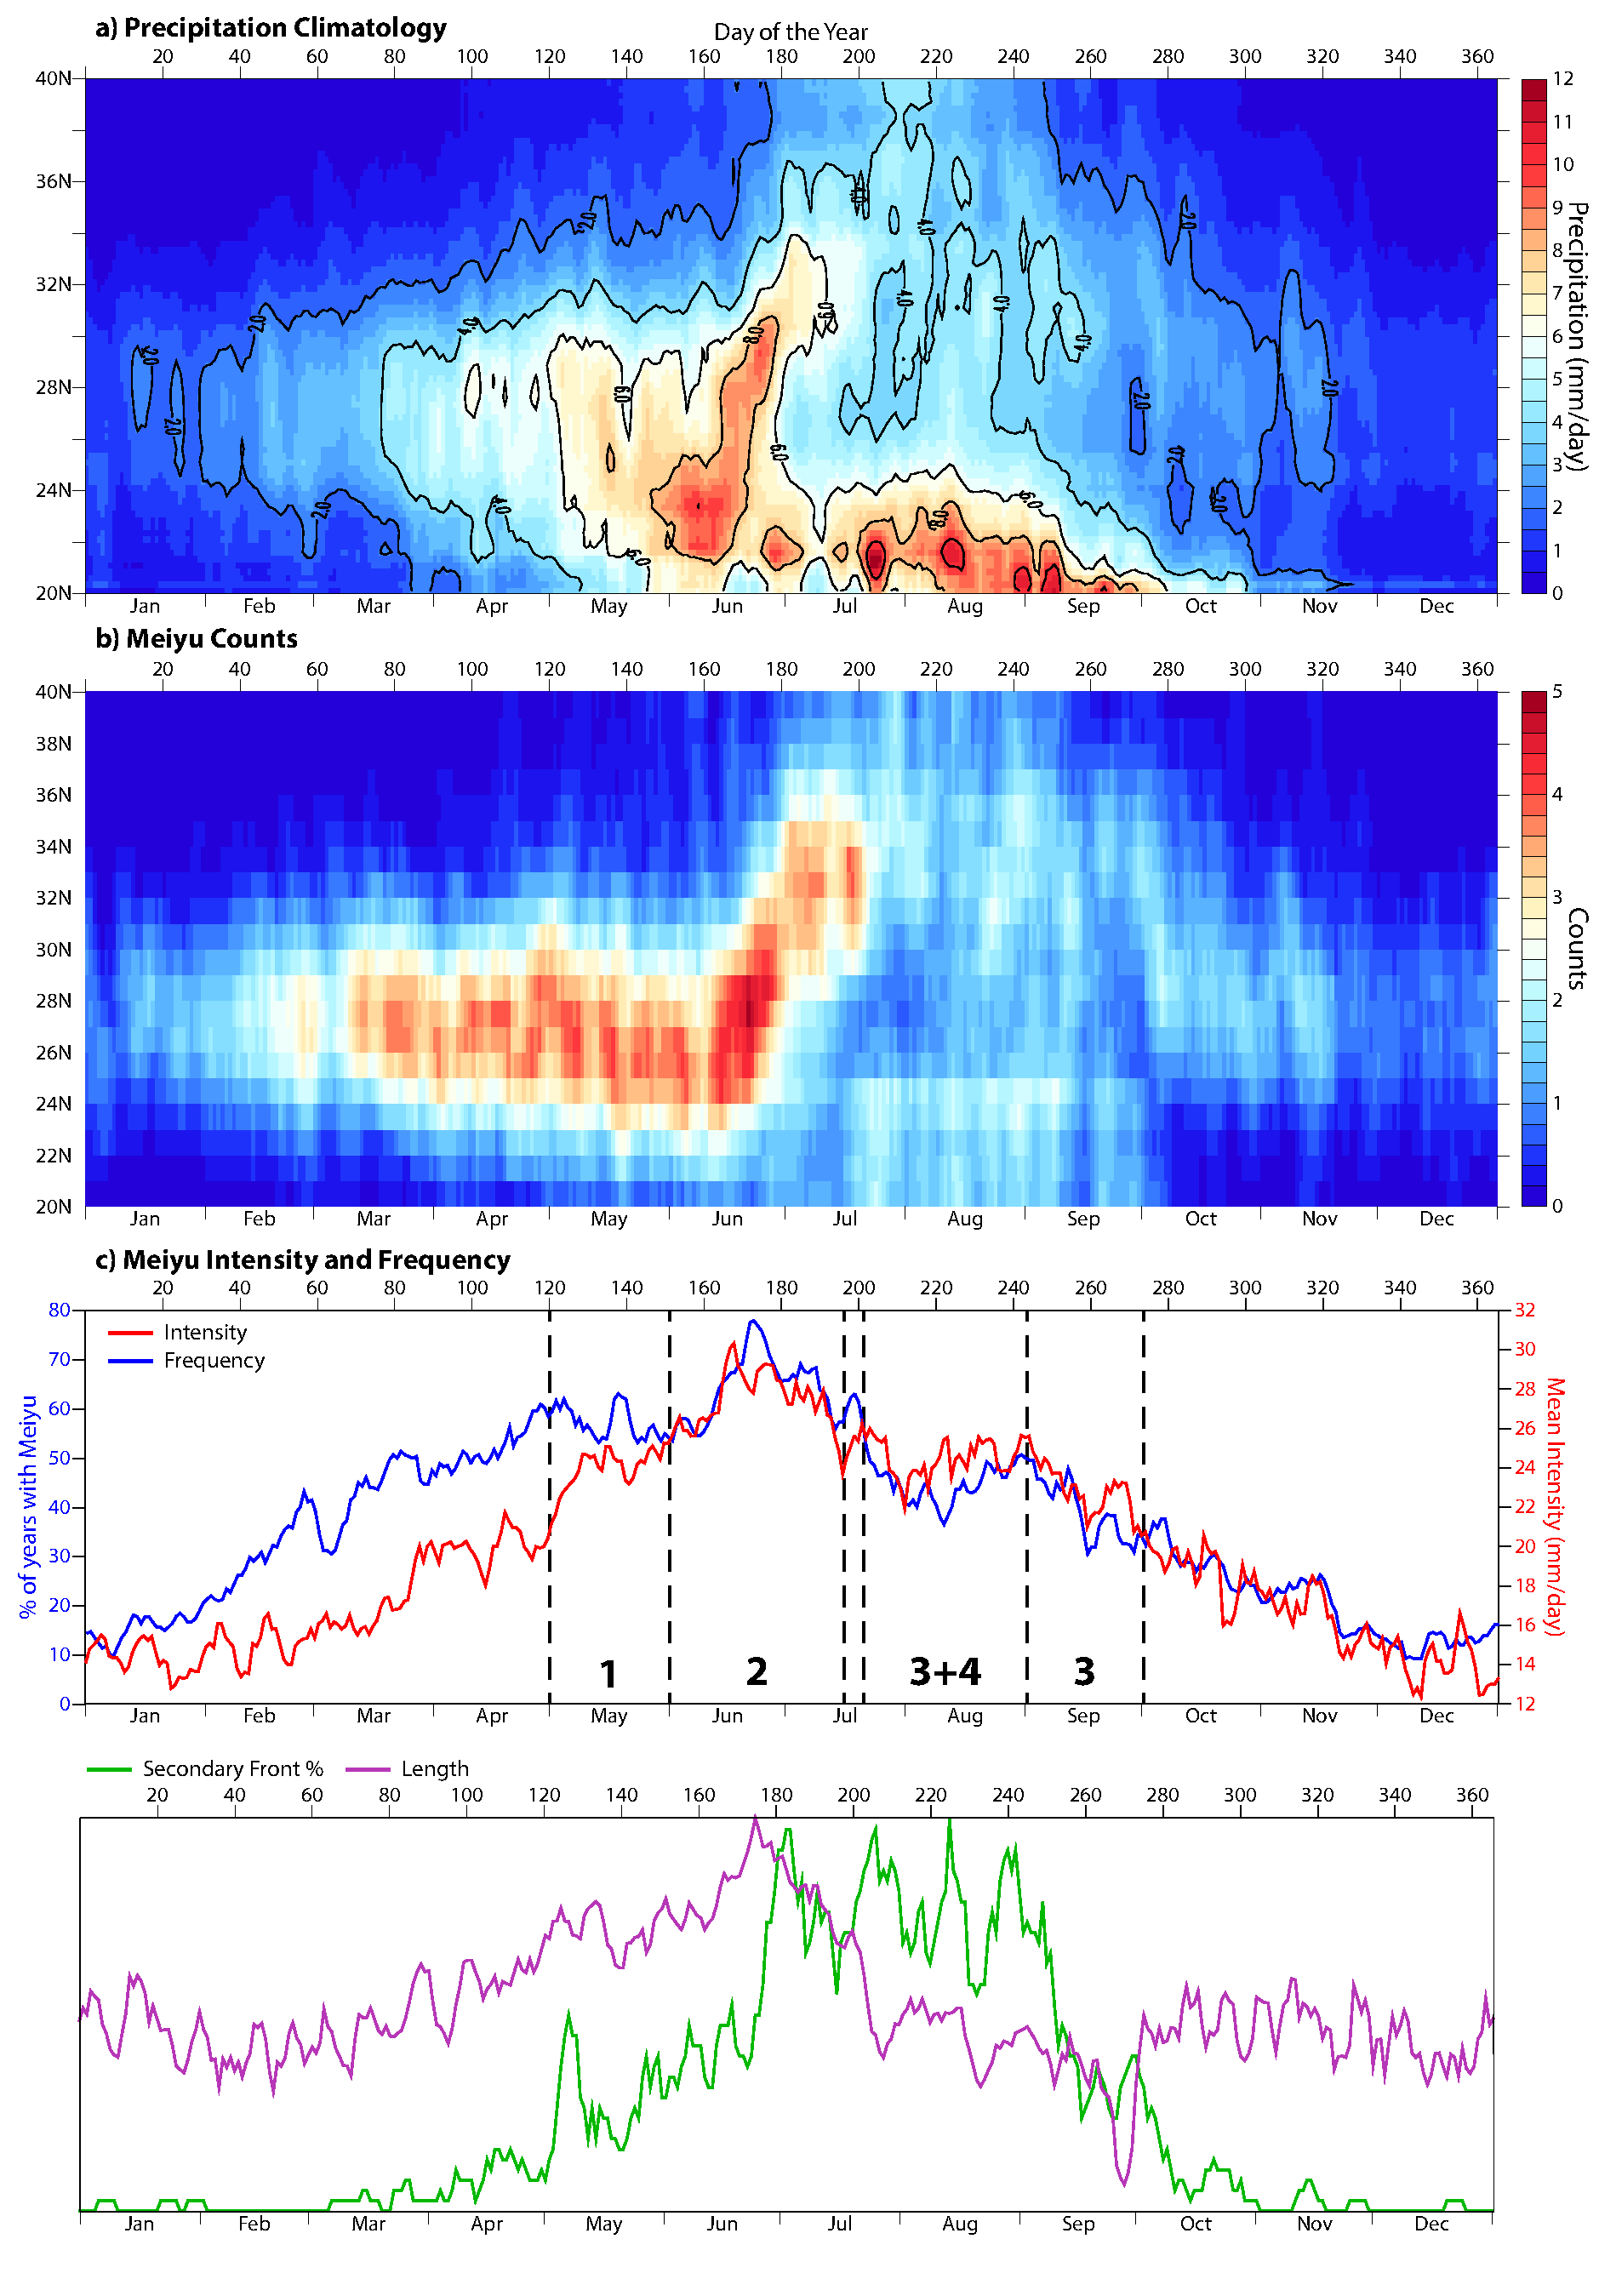
\includegraphics[width=36pc]{Figures/fig1_dingchan.pdf}
\caption{Climatology of the Meiyu Front, 1951-2007. 1) Pre-Meiyu 2) Meiyu 3) Cyclone season in Southern China 4) Storms advected by summer jet}
\label{dingchan}
\end{figure}


%%% Changes in jet mean between 1951-1979 and 1980-2007
\begin{figure}[htbp]
\begin{center}
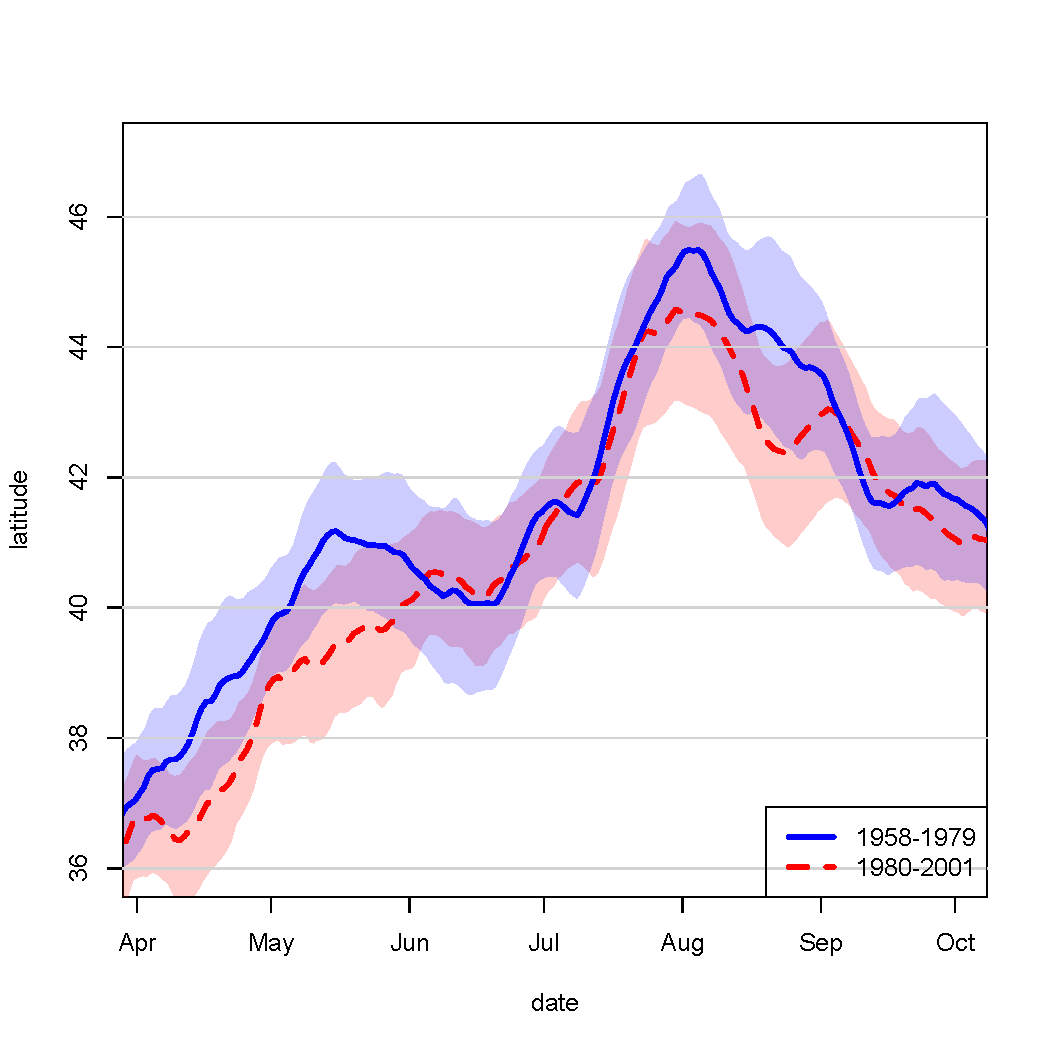
\includegraphics[width=5in]{Figures/jet_seasonal.pdf}
\caption{7-day running mean latitude of the westerly jet in the region 90-130$^\circ$E for the 1958-1979 (blue, solid) and 1980-2001 (red, dashed). Bootstrapped 95\% confidence intervals are shaded. }
\label{jet_seasonal}
\end{center}
\end{figure}

%%% Changes in Meiyu and rainfall behavior between 1951-1979 and 1980-2007
\begin{figure}[htbp]
\begin{center}
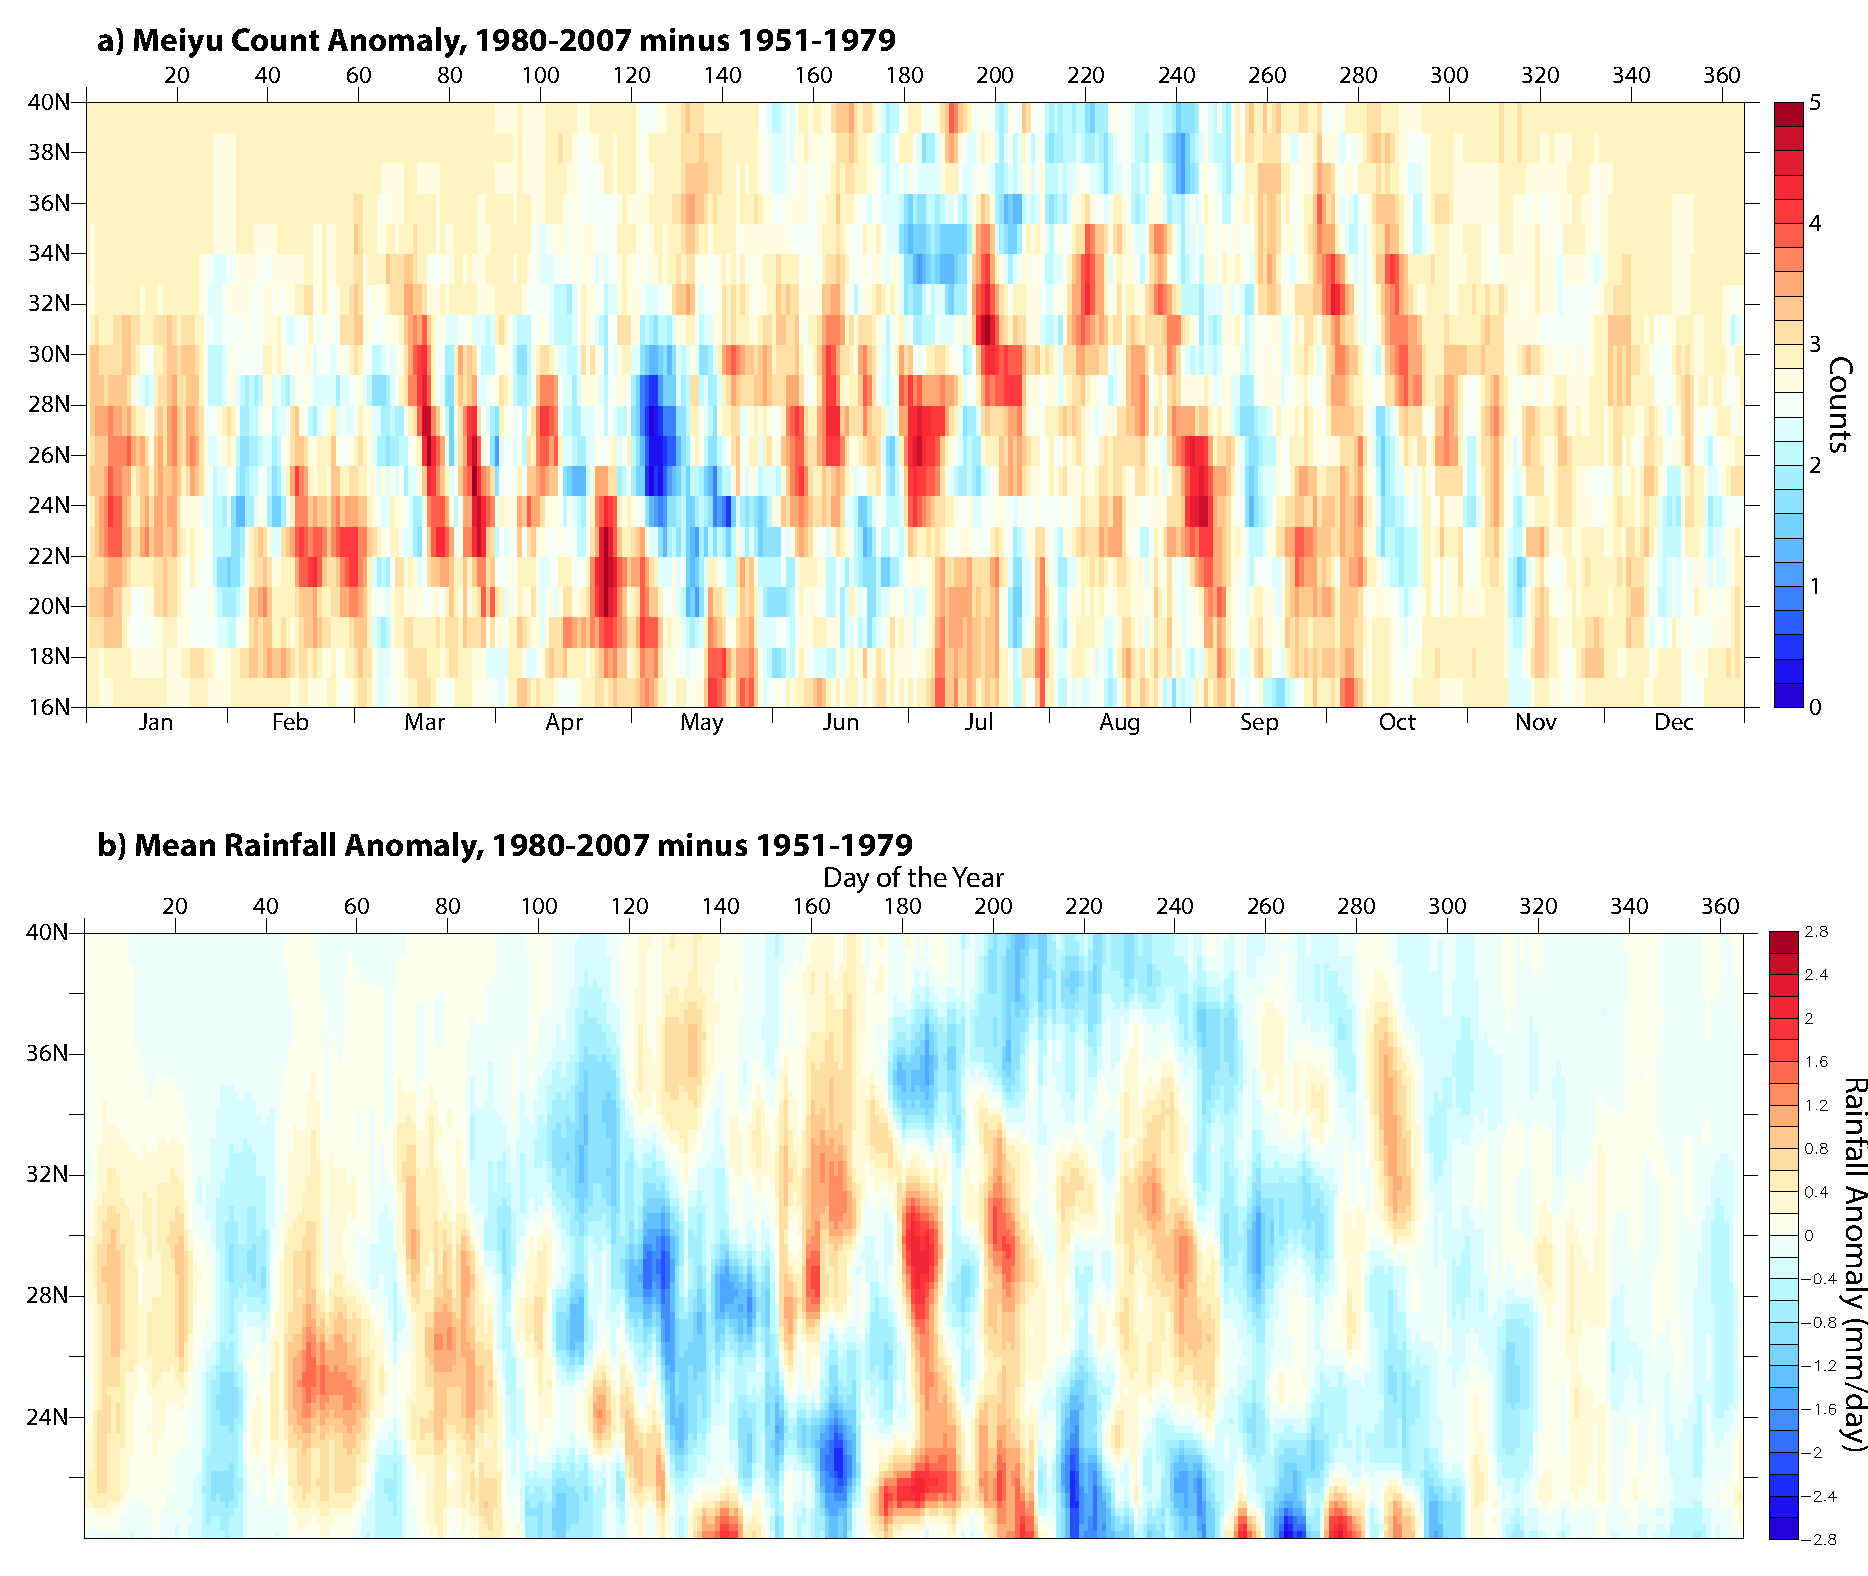
\includegraphics[width=36pc]{Figures/fig3_changes.pdf}
\caption{a) Change in rainfall between 1951-1979 and 1980-07, with 95\%/99\% confidence level marked by single/double cross-hatches. b) Change in Meiyu front frequency between 1951-1979 and 1980-07, with confidence levels marked as in a).}
\label{changes}
\end{center}
\end{figure}


%%%% TABLE 1 - MEIYU STATISTICS %%%%

\begin{table}
\caption{Frequency of primary and secondary fronts, as well as latitude and intensity during the Spring rains, pre-Meiyu, Meiyu season, post-Meiyu, and for the full year. These variables are calculated over the years 1951-2007, 1951-1979 and 1980-2007. Statistically significant differences between 1951-1979 and 1980-2007 at the 95\%/99\% level are indicated by bold/bold and italic, as calculated by a permutation method and a bootstrapping method described in the main text.}
\centering

\begin{tabular}{ l c c c c}
	 \multicolumn{5}{c}{\textbf{1951-2007}} \\
	 \textbf{Time Period} & \textbf{1ff.} (\%) &\textbf{2ff.} (\%) & \textbf{Lat} & \textbf{Int} (mm day$^{-1}$) \\
	 \hline
	\textbf{Spring} (81-120) & $50.9 \pm 1.0$ & $1.0 \pm 0.2$ & $27.2$ & 21.1 \\
	\textbf{Pre-Meiyu} (121-155) & $56.5 \pm 1.1$ & $3.7 \pm 0.4$ & $27.0$ & 25.8 \\
	\textbf{Meiyu I} (156-180) &	$65.2 \pm 1.3$ & $6.2 \pm 0.6$ & $27.7$ & 30.0 \\
	\textbf{Meiyu II} (181-200) & $63.2 \pm 1.4$ & $10.3 \pm 0.9$ & $31.0$ & 28.5 \\
	\textbf{Meiyu} (156-200) & $64.3 \pm 0.9$ & $8.1 \pm 0.5$ & $29.1$ & 29.3 \\
	\textbf{Post-Meiyu} (201-270) & $42.7 \pm 0.8 $ & $8.7 \pm 0.4$ & $29.6$ & 26.8 \\
	\textbf{Whole Year} (1-365) & $38.4 \pm 0.3$ & $3.3 \pm 0.1$ & $28.3$ & 23.8 \\
\end{tabular}

\begin{tabular}{ l c c c c c c}
	& \multicolumn{3}{c}{\textbf{1951-1979}} & \multicolumn{3}{c}{\textbf{1980-2007}} \\
	\textbf{Period} & 1\% & 2\% & L & 1\% & 2\% & L \\
	\hline	
	\textbf{Spring} (81-120) & $50.6 \pm 1.5$ & $1.0 \pm 0.3$ & $\boldsymbol{27.4 \pm .2^*}$ & $51.2 \pm 1.5$ & $1.1 \pm 0.3$ & $\boldsymbol{27.0 \pm 0.2^*}$ \\
	\textbf{Pre-Meiyu} (121-155) & $\boldsymbol{60.7 \pm 1.5^*}$ & $3.8 \pm 0.6$ & $27.1 \pm .2$ & $\boldsymbol{52.2 \pm 1.6^*}$ & $3.6 \pm 0.6$ & $26.9 \pm 0.3$ \\
	\textbf{Meiyu I} (156-180) &	$65.7 \pm 1.8$ & $5.8 \pm 0.9$ & $27.6 \pm .3$ & $64.7 \pm 1.8$  & $6.7 \pm 0.9$ & 6$ 27.9 \pm 0.3$ \\
	\textbf{Meiyu II} (181-200) & $63.4 \pm 2.0$ & $9.3 \pm 1.2$ & $31.1 \pm .4$ & $63.0 \pm 2.0$ & $11.4 \pm 1.3$ & $30.7 \pm 0.3$ \\
	\textbf{Meiyu} (156-200) & $64.7 \pm 7.4$ & $0.7 \pm 0.7$ & $29.2 \pm .3$ & $64.0 \pm 1.4$ & $8.8 \pm .8$ & $29.1 \pm 0.3$ \\
	\textbf{Post-Meiyu} (201-270) & $43.0 \pm 1.1 $ & $9.4 \pm 0.6$ & $\boldsymbol{29.9 \pm .3}$ & $42.2 \pm 1.1$ & $8.0 \pm 0.6$ & $\boldsymbol{29.3 \pm 0.4}$  \\
	\textbf{Whole Year} (1-365) & $38.6 \pm 0.5 $ & $3.4 \pm 0.2 $ & $\boldsymbol{28.4 \pm .1}$ & $38.1 \pm 0.5$ & $3.3 \pm 0.2$ & $\boldsymbol{28.2 \pm 0.1} $ \\
\end{tabular}

\begin{tabular}{ l c c c c c c c c}
	& \multicolumn{3}{c}{\textbf{1951-1979}} & \multicolumn{3}{c}{\textbf{1980-2007}} \\
	\textbf{Period} & 1\% & 2\% & L & I & 1\% & 2\% & L & I \\
	\hline	
	\textbf{Spring} (81-120) & $50.6 \pm 1.5$ & $1.0 \pm 0.3$ & $\boldsymbol{27.4 \pm .2^*}$ & $20.8 \pm .7$ & $51.2 \pm 1.5$ & $1.1 \pm 0.3$ & $\boldsymbol{27.0 \pm 0.2^*}$ & $21.4 \pm .7$ \\
	\textbf{Pre-Meiyu} (121-155) & $\boldsymbol{60.7 \pm 1.5^*}$ & $3.8 \pm 0.6$ & $27.1 \pm .2$ & $25.6 \pm .8$ & $\boldsymbol{52.2 \pm 1.6^*}$ & $3.6 \pm 0.6$ & $26.9 \pm 0.3$ & $26.0 \pm .8$\\
	\textbf{Meiyu I} (156-180) &	$65.7 \pm 1.8$ & $5.8 \pm 0.9$ & $27.6 \pm .3$ & $30.2 \pm 1.0$ & $64.7 \pm 1.8$  & $6.7 \pm 0.9$ & 6$ 27.9 \pm 0.3$ & $29.8 \pm 1.0$ \\
	\textbf{Meiyu II} (181-200) & $63.4 \pm 2.0$ & $9.3 \pm 1.2$ & $31.1 \pm .4$ & $27.9 \pm 1.1$ & $63.0 \pm 2.0$ & $11.4 \pm 1.3$ & $30.7 \pm 0.3$ & $29.1 \pm 1.1$ \\
	\textbf{Meiyu} (156-200) & $64.7 \pm 7.4$ & $0.7 \pm 0.7$ & $29.2 \pm .3$ & $29.2 \pm .7$ & $64.0 \pm 1.4$ & $8.8 \pm .8$ & $29.1 \pm 0.3$ & $29.5 \pm .8$\\
	\textbf{Post-Meiyu} (201-270) & $43.0 \pm 1.1 $ & $9.4 \pm 0.6$ & $\boldsymbol{29.9 \pm .3}$ & $26.7 \pm .8$ & $42.2 \pm 1.1$ & $8.0 \pm 0.6$ & $\boldsymbol{29.3 \pm 0.4}$ &  $26.8 \pm .8$ \\
	\textbf{Whole Year} (1-365) & $38.6 \pm 0.5 $ & $3.4 \pm 0.2 $ & $\boldsymbol{28.4 \pm .1}$ & $23.7 \pm .3$ & $38.1 \pm 0.5$ & $3.3 \pm 0.2$ & $\boldsymbol{28.2 \pm 0.1} $ & $24.0 \pm .3$\\
\end{tabular}

%\begin{tabularx}{.9\textwidth}{ >{\setlength\hsize{.075X@{}\hsize}\centering}X@{} >{\setlength\hsize{.075\hsize}\centering}X@{} >{\setlength\hsize{.075\hsize}\centering}X@{} >{\setlength\hsize{.075\hsize}\centering}X@{} >{\setlength\hsize{.075\hsize}\centering}X@{} >{\setlength\hsize{.075\hsize}\centering}X@{} >{\setlength\hsize{.075\hsize}\centering}X@{} >{\setlength\hsize{.075\hsize}\centering}X@{} >{\setlength\hsize{.075\hsize}\centering}X@{} >{\setlength\hsize{.075\hsize}\centering}X@{} >{\setlength\hsize{.075\hsize}\centering}X@{} >{\setlength\hsize{.075\hsize}\centering}X@{} }
%\hline
 %\multicolumn{4}{>{\setlength\hsize{.3\hsize}\centering } X}{1951-2007}  &  \multicolumn{4}{>{\setlength\hsize{.3\hsize}\centering } X}{1951-1979} \multicolumn{4}{>{\setlength\hsize{.3\hsize}\centering } X}{1980-2007}  \tabularnewline
%\end{tabularx}
\label{changes_table}
\end{table}

\end{document}

%% ------------------------------------------------------------------------ %%
%
%  SECTION HEADS
%
%% ------------------------------------------------------------------------ %%

% Capitalize the first letter of each word (except for
% prepositions, conjunctions, and articles that are
% three or fewer letters).

% AGU follows standard outline style; therefore, there cannot be a section 1 without
% a section 2, or a section 2.3.1 without a section 2.3.2.
% Please make sure your section numbers are balanced.
% ---------------
% Level 1 head
%
% Use the \section{} command to identify level 1 heads;
% type the appropriate head wording between the curly
% brackets, as shown below.
%
%An example:
%\section{Level 1 Head: Introduction}
%
% ---------------
% Level 2 head
%
% Use the \subsection{} command to identify level 2 heads.
%An example:
%\subsection{Level 2 Head}
%
% ---------------
% Level 3 head
%
% Use the \subsubsection{} command to identify level 3 heads
%An example:
%\subsubsection{Level 3 Head}
%
%---------------
% Level 4 head
%
% Use the \subsubsubsection{} command to identify level 3 heads
% An example:
%\subsubsubsection{Level 4 Head} An example.
%
%% ------------------------------------------------------------------------ %%
%
%  IN-TEXT LISTS
%
%% ------------------------------------------------------------------------ %%
%
% Do not use bulleted lists; enumerated lists are okay.
% \begin{enumerate}
% \item
% \item
% \item
% \end{enumerate}
%



%% ------------------------------------------------------------------------ %%
%
%  SIDEWAYS FIGURE AND TABLE EXAMPLES
%
%% ------------------------------------------------------------------------ %%
%
% For tables and figures, add \usepackage{rotating} to the paper and add the rotating.sty file to the folder.
% AGU prefers the use of {sidewaystable} over {landscapetable} as it causes fewer problems.
%
% \begin{sidewaysfigure}
% \includegraphics[width=20pc]{samplefigure.eps}
% \caption{caption here}
% \label{label_here}
% \end{sidewaysfigure}
%
%
%
% \begin{sidewaystable}
% \caption{}
% \begin{tabular}
% Table layout here.
% \end{tabular}
% \end{sidewaystable}
%
%

